\documentclass[10pt]{article}
\usepackage[polish]{babel}
\usepackage[utf8]{inputenc}
\usepackage[T1]{fontenc}
\usepackage{amsmath}
\usepackage{amsfonts}
\usepackage{amssymb}
\usepackage[version=4]{mhchem}
\usepackage{stmaryrd}
\usepackage{graphicx}
\usepackage[export]{adjustbox}
\graphicspath{ {./images/} }

\newcommand\Varangle{\mathop{{<\!\!\!\!\!\text{\small)}}\:}\nolimits}

\begin{document}
\begin{enumerate}
  \item Rozwiąż w liczbach całkowitych równanie:
\end{enumerate}

\[
x(x+1)(x+2)+(x+1)(x+2)(x+3)+\cdots+(x+98)(x+99)(x+100)=2019 x+2020
\]

\begin{enumerate}
  \setcounter{enumi}{1}
  \item Znajdź wszystkie pary liczb całkowitych \(x, y\) spełniających równanie
\end{enumerate}

\[
x^{2}+y^{2}=16848
\]

\begin{enumerate}
  \setcounter{enumi}{2}
  \item W prostokącie \(A B C D\) punkty \(E\) i \(F\) leżą odpowiednio na bokach \(B C\) i \(C D\), przy czym \(\Varangle E A F=45^{\circ}\) oraz \(B E=D F\). Wykaż, że pole trójkąta \(A E F\) jest równe sumie pól trójkątów \(A B E\) i \(A D F\).\\
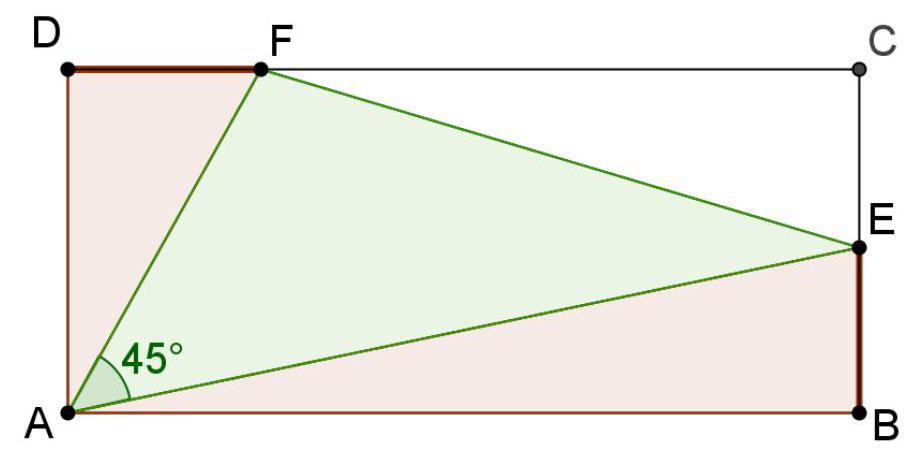
\includegraphics[max width=\textwidth, center]{2024_11_21_98438ec859db2c8405cag-1}
\end{enumerate}

\end{document}